Στο σχήμα \ref{fig:02_05_04:02} απεικονίζεται η διαδικασία ευθυγράμμισης δύο
πανοραμικών δισδιάστατων σαρώσεων που συνελήθησαν σε ένα περιβάλλον του συνόλου
δεδομένων \texttt{laserazos}\footref{foot:laserazos} μέσω των μεθόδων FastGICP
και FSM.  Εδώ παρατηρούμε πως ο πρώτος---όπως και όλες οι εκδόσεις του
ICP---εκτιμούν σταδιακά τον προσανατολισμό ανάμεσα στις δύο στάσεις από τις
οποίες συνελήφθησαν οι δύο σαρώσεις, σε αντίθεση με τον FSM, ο οποίος το κάνει
σε ένα βήμα---από εκεί και πέρα παρέχει όλο και πιο ακριβείς εκτιμήσεις μέσω
της υπερδειγματοληψίας του χάρτη $\widetilde{\bm{M}}$. Ο FastGICP χρησιμοποιεί
αντιστοιχίσεις για τα δύο σκέλη της ευθυγράμμισης, και ως εσωτερική μετρική το
μέτρο της εξ. (\ref{eq:sm_def}), ενώ ο FSM δεν χρησιμοποιεί αντιστοιχίσεις
όλως διόλου, και η εσωτερική μετρική του είναι η μετρική CAER (εξ.
(\ref{eq:caer_normal}), όπου $\mathcal{S}_R \leftarrow \mathcal{S}_1$,
$\mathcal{S}_V \leftarrow \mathcal{S}_0$, $(x,y,\theta)\leftarrow\bm{p}_1$, και
$(\hat{x}, \hat{y}, \hat{\theta}) \leftarrow \bm{p}_0$). Από τα αποτελέσματα
παρατηρούμε πως το σφάλμα εκτίμησης θέσης του FastGICP δεν ακολουθεί την
(μειούμενη) τροχιά της εσωτερικής του μετρικής---σε αντίθεση με αυτό του
FSM---και πως αυξάνει προτού στη συνέχεια μειωθεί, με αποτέλεσμα την
παγίδευση της εκτίμησης θέσης σε τοπικό ελάχιστο. Δεδομένου ότι οι συχνότητα
ανανέωσης μετρήσεων από τους εμπορικά διαθέσιμους πανοραμικούς αισθητήρες lidar
κυμαίνεται από $10$-$20$ Hz, με βάση την απόσταση των στάσεων από τις οποίες
συνελήφθησαν οι δύο μετρήσεις, συμπεραίνουμε πως ο FSM είναι ικανός εκτίμησης
της τροχιάς ενός ρομπότ το οποίο κινείται με ακτινική ταχύτητα $7.28$ m/s
($\approx 25$ km/h), και γωνιακή ταχύτητα $6\pi$ rad/s.

\begin{figure}[]\centering
  \input{./figures/parts/02/chapters/05/sections/04/fsm_vs_fgi.tex}
  \vspace{0.5cm}
  \caption{\small Η εξέλιξη της διαδικασίας ευθυγράμμισης των δύο σαρώσεων του
           σχήματος της άνω σειράς μέσω του FastGICP (αριστερά) και του
           FSM (δεξιά). Οι δύο σαρώσεις διαταράσσονται από θόρυβο
           $\mathcal{N} \sim (0, 0.03^2)$ [m, m$^2$] και συλλαμβάνονται από
           στάσεις με διαφορά $\Delta = (0.35, 0.10, -\pi/3)$ [m,m,rad].
           Τα τελικά σφάλματα θέσης και προσανατολισμού του FastGICP είναι
           $0.61$ m και $0.173$ rad αντίστοιχα, ενώ του FSM
           $0.0098$ m και $0.0014$ rad}
  \label{fig:02_05_04:02}
\end{figure}


Στο σχήμα \ref{fig:02_05_04:01} απεικονίζεται η χρησιμότητα της ευθυγράμμισης
σαρώσεων: σε συνθήκες απουσίας χάρτη του περιβάλλοντος (όπως π.χ. κατά την
επίλυση του προβλήματος SLAM) μία μέθοδος ευθυγράμμισης σαρώσεων δρα ως
παρατηρητής της στάσης ενός ρομπότ. Στο πρόβλημα της ευθυγράμμισης πραγματικών
με εικονικές σαρώσεις (κεφ. \ref{part:02:chapter:04}) ο χάρτης δρα ως μέσο
ανάδρασης λόγω της αντιστοιχίας του με το περιβάλλον και του σταθερού
συστήματος αναφοράς που ο ίδιος παρέχει---η απουσία του εδώ, συνεπώς, αφαιρεί
και τη δυνατότητα φραγής του σφάλματος εκτίμησης.\footnote{Η ίδια απουσία
σταθερού συστήματος αναφοράς βαραίνει και την εκτίμηση της στάσης του ρομπότ
μέσω κωδικοποιητών.} Στο σχήμα \ref{fig:02_05_04:01} παρατηρούμε πως σε
ιδανικές συνθήκες ($\sigma_R = 0.0$ m) οι PLICP και NDT εισάγουν οι ίδιες
σφάλματα εκτίμησης---πιθανότατα λόγω αποστάσεων θέσης και προσανατολισμού με
μέτρο μεγαλύτερο από ότι μπορούν να διορθώσουν με μεγαλύτερη ακρίβεια. Σε
συνθήκες όπου ο αισθητήρας λαμβάνει αραιότερα δείγματα στο χώρο αυτές οι
αποστάσεις αυξάνουν, με αποτέλεσμα αυξημένα σφάλματα. Σε αντίθεση ο
FSM είναι ικανός να παρατηρήσει την τροχιά του αισθητήρα με μεγαλύτερη
ακρίβεια.

\begin{figure}[]\centering
  \definecolor{aa}{RGB}{227,26,28}
\definecolor{ab}{RGB}{56,125,184}
\definecolor{ac}{RGB}{77,176,74}
\definecolor{ak}{RGB}{0,0,0}

% GNUPLOT: LaTeX picture with Postscript
\begingroup
  \makeatletter
  \providecommand\color[2][]{%
    \GenericError{(gnuplot) \space\space\space\@spaces}{%
      Package color not loaded in conjunction with
      terminal option `colourtext'%
    }{See the gnuplot documentation for explanation.%
    }{Either use 'blacktext' in gnuplot or load the package
      color.sty in LaTeX.}%
    \renewcommand\color[2][]{}%
  }%
  \providecommand\includegraphics[2][]{%
    \GenericError{(gnuplot) \space\space\space\@spaces}{%
      Package graphicx or graphics not loaded%
    }{See the gnuplot documentation for explanation.%
    }{The gnuplot epslatex terminal needs graphicx.sty or graphics.sty.}%
    \renewcommand\includegraphics[2][]{}%
  }%
  \providecommand\rotatebox[2]{#2}%
  \@ifundefined{ifGPcolor}{%
    \newif\ifGPcolor
    \GPcolorfalse
  }{}%
  \@ifundefined{ifGPblacktext}{%
    \newif\ifGPblacktext
    \GPblacktexttrue
  }{}%
  % define a \g@addto@macro without @ in the name:
  \let\gplgaddtomacro\g@addto@macro
  % define empty templates for all commands taking text:
  \gdef\gplfronttext{}%
  \gdef\gplfronttext{}%
  \makeatother
  \ifGPblacktext
    % no textcolor at all
    \def\colorrgb#1{}%
    \def\colorgray#1{}%
  \else
    % gray or color?
    \ifGPcolor
      \def\colorrgb#1{\color[rgb]{#1}}%
      \def\colorgray#1{\color[gray]{#1}}%
      \expandafter\def\csname LTw\endcsname{\color{white}}%
      \expandafter\def\csname LTb\endcsname{\color{black}}%
      \expandafter\def\csname LTa\endcsname{\color{black}}%
      \expandafter\def\csname LT0\endcsname{\color[rgb]{1,0,0}}%
      \expandafter\def\csname LT1\endcsname{\color[rgb]{0,1,0}}%
      \expandafter\def\csname LT2\endcsname{\color[rgb]{0,0,1}}%
      \expandafter\def\csname LT3\endcsname{\color[rgb]{1,0,1}}%
      \expandafter\def\csname LT4\endcsname{\color[rgb]{0,1,1}}%
      \expandafter\def\csname LT5\endcsname{\color[rgb]{1,1,0}}%
      \expandafter\def\csname LT6\endcsname{\color[rgb]{0,0,0}}%
      \expandafter\def\csname LT7\endcsname{\color[rgb]{1,0.3,0}}%
      \expandafter\def\csname LT8\endcsname{\color[rgb]{0.5,0.5,0.5}}%
    \else
      % gray
      \def\colorrgb#1{\color{black}}%
      \def\colorgray#1{\color[gray]{#1}}%
      \expandafter\def\csname LTw\endcsname{\color{white}}%
      \expandafter\def\csname LTb\endcsname{\color{black}}%
      \expandafter\def\csname LTa\endcsname{\color{black}}%
      \expandafter\def\csname LT0\endcsname{\color{black}}%
      \expandafter\def\csname LT1\endcsname{\color{black}}%
      \expandafter\def\csname LT2\endcsname{\color{black}}%
      \expandafter\def\csname LT3\endcsname{\color{black}}%
      \expandafter\def\csname LT4\endcsname{\color{black}}%
      \expandafter\def\csname LT5\endcsname{\color{black}}%
      \expandafter\def\csname LT6\endcsname{\color{black}}%
      \expandafter\def\csname LT7\endcsname{\color{black}}%
      \expandafter\def\csname LT8\endcsname{\color{black}}%
    \fi
  \fi
    \setlength{\unitlength}{0.0500bp}%
    \ifx\gptboxheight\undefined%
      \newlength{\gptboxheight}%
      \newlength{\gptboxwidth}%
      \newsavebox{\gptboxtext}%
    \fi%
    \setlength{\fboxrule}{0.5pt}%
    \setlength{\fboxsep}{1pt}%
\begin{picture}(5000.00,5000.00)%
    \gplgaddtomacro\gplfronttext{%
      \colorrgb{0.15,0.15,0.15}%
      \put(391,1564){\makebox(0,0)[r]{\strut{}$6.0$}}%
      \colorrgb{0.15,0.15,0.15}%
      \put(391,1988){\makebox(0,0)[r]{\strut{}$8.0$}}%
      \colorrgb{0.15,0.15,0.15}%
      \put(391,2413){\makebox(0,0)[r]{\strut{}$10.0$}}%
      \colorrgb{0.15,0.15,0.15}%
      \put(391,2837){\makebox(0,0)[r]{\strut{}$12.0$}}%
      \colorrgb{0.15,0.15,0.15}%
      \put(391,3262){\makebox(0,0)[r]{\strut{}$14.0$}}%
      \colorrgb{0.15,0.15,0.15}%
      \put(391,3687){\makebox(0,0)[r]{\strut{}$16.0$}}%
      \colorrgb{0.00,0.00,0.00}%
      \put(672,1280){\makebox(0,0){\strut{}$-2.0$}}%
      \colorrgb{0.00,0.00,0.00}%
      \put(1096,1280){\makebox(0,0){\strut{}$0.0$}}%
      \colorrgb{0.00,0.00,0.00}%
      \put(1521,1280){\makebox(0,0){\strut{}$2.0$}}%
      \colorrgb{0.00,0.00,0.00}%
      \put(1945,1280){\makebox(0,0){\strut{}$4.0$}}%
      \colorrgb{0.00,0.00,0.00}%
      \put(2370,1280){\makebox(0,0){\strut{}$6.0$}}%

      \put(1020,4104){\makebox(0,0){\strut{}{\color{ak}{\rule[0.6mm]{0.5cm}{0.5mm}}} \small Τροχιά αισθητήρα}}
      \put(2570,4104){\makebox(0,0){\strut{}{\color{aa}{\rule[0.6mm]{0.5cm}{0.5mm}}} \small PLICP}}
      \put(3500,4104){\makebox(0,0){\strut{}{\color{ab}{\rule[0.6mm]{0.5cm}{0.5mm}}} \small NDT}}
      \put(4440,4104){\makebox(0,0){\strut{}{\color{ac}{\rule[0.6mm]{0.5cm}{0.5mm}}} \small \texttt{fsm}}}
      \put(1500,1004){\makebox(0,0){\strut{} \small Πυκνές μετρήσεις}}
      \put(3600,1004){\makebox(0,0){\strut{} \small Αραιές μετρήσεις}}
    }%
    \gplgaddtomacro\gplfronttext{%
    }%
    \gplgaddtomacro\gplfronttext{%
      \colorrgb{0.00,0.00,0.00}%
      \put(2822,1280){\makebox(0,0){\strut{}$-2.0$}}%
      \colorrgb{0.00,0.00,0.00}%
      \put(3246,1280){\makebox(0,0){\strut{}$0.0$}}%
      \colorrgb{0.00,0.00,0.00}%
      \put(3671,1280){\makebox(0,0){\strut{}$2.0$}}%
      \colorrgb{0.00,0.00,0.00}%
      \put(4095,1280){\makebox(0,0){\strut{}$4.0$}}%
      \colorrgb{0.00,0.00,0.00}%
      \put(4520,1280){\makebox(0,0){\strut{}$6.0$}}%
    }%
    \gplgaddtomacro\gplfronttext{%
    }%
    \put(0,0){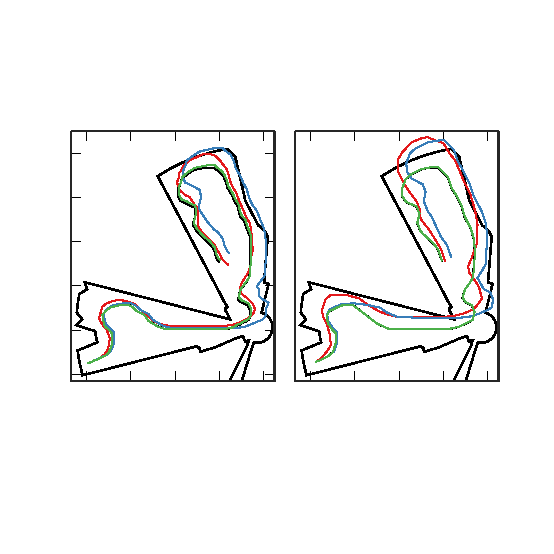
\includegraphics{./figures/parts/02/chapters/05/sections/04/odom_test_5_vs_6}}%
    \gplfronttext
  \end{picture}%
\endgroup

  \vspace{-2cm}
  \caption{\small Η ευθυγράμμιση σαρώσεων ως μέσο παρατήρησης της τροχιάς του
           αισθητήρα, ή αλλιώς ως ``laser odometry": το ρομπότ κινείται από
           την κάτω αριστερά περιοχή του περιβάλλοντος προς την άνω δεξιά,
           συλλαμβάνοντας μετρήσεις καθ' οδόν. Οι χρωματισμένες γραμμές
           απεικονίζουν τις εκτιμώμενες τροχιές του αισθητήρα από κάθε μέθοδο.
           Ο FSM διατηρεί την ακρίβειά του σε συνθήκες αραιούς χωρικά
           δειγματοληψίας λόγω της ικανότητάς του να διοθρώνει ``μεγάλες"
           αποστάσεις μεταξύ θέσεων, και λόγω της αναλλοιωσιμότητας της
           ικανότητας εκτίμησης προσανατολισμού κατά μήκος όλων των δυνατών
           προσανατολισμών. Τα σφάλματα εκτίμησης του FSM κατά μήκος
           της τροχιάς του αισθητήρα είναι μεγαλύτερα σε συνθήκες πυκνής
           δειγματοληψίας από ότι σε συνθήκες αραιούς (σε αντίθεση με αυτά των
           PLICP και NDT) λόγω της ενσωμάτωσης περισσότερων εκτιμήσεων (και
           συνεπώς περισσότερων σφαλμάτων εκτίμησης)}
  \label{fig:02_05_04:01}
\end{figure}


Οι κύριοι περιορισμοί της απόκρισης των μεθόδων ευθυγράμμισης σαρώσεων είναι οι
ίδιοι με αυτούς των προσθετικών μεθόδων ευθυγράμμισης πραγματικών με εικονικές
σαρώσεις. Αυτοί αφορούν στα αμετάβλητα χαρακτηριστικά μεγέθη του φυσικού
αισθητήρα σαρώσεων, τα οποία είναι δυο. Το πρώτο είναι το μέγεθος των
διαταραχών που επιδρούν στις μετρήσεις του, την απόκριση επί του οποίου
εξετάσαμε για διάφορες τιμές στην ενότητα \ref{section:02_05_03}. Το δεύτερο
είναι το βεληνεκές του αισθητήρα, δηλαδή η μέγιστη απόσταση μέχρι την οποία
μπορεί να ανιχνεύσει την παρουσία αντικειμένων.

Στην άνω σειρά του σχήματος \ref{fig:02_05_04:03} εμφανίζονται με λευκό χρώμα
δύο διαφορετικά περιβάλλοντα, μέσα στα οποία τοποθετείται ένας αισθητήρας στις
θέσεις που σημειώνονται με κουκκίδες βαθύ μπλε χρώματος. Οι θέσεις αυτές είναι
τα κέντρα των ομόκεντρων κύκλων που εμφανίζονται στην ίδια σειρά. Η πειραματική
διάταξη που ακολουθεί στοχεύει στην καταγραφή της απόκρισης των μεθόδων
PLICP και FSM σε πειράματα όπου το βεληνεκές του αισθητήρα
μεταβάλλεται έτσι ώστε οι μετρήσεις του να περιλαμβάνουν όλα τα εμπόδια του
περιβάλλοντος, μειούμενο μέχρι που να μην περιλαμβάνουν κανένα. Το βεληνεκές
του αισθητήρα είναι η ακτίνα των κύκλων της πρώτης σειράς του σχήματος, και το
χρώμα αυτών αναπαριστά το ποσοστό των ακτίνων που φέρουν χωρική πληροφορία,
βάσει της χρωματικής λωρίδας που παρουσιάζεται στη δεύτερη σειρά. Στις δύο
τελευταίες σειρές παρατίθενται οι μέσοι όροι των σφαλμάτων εκτίμησης
προσανατολισμού και θέσης σε δέκα επαναλήψεις, για κάθε μέθοδο και περιβάλλον,
για $\sigma_R = 0.05$ m. Η δεύτερη στάση του αισθητήρα παράγεται τυχαία για
κάθε πείραμα μέσω διαταραχής των αντίστοιχων συνιστωσών της πρώτης στάσης του
αισθητήρα με ποσότητες που εξάγονται από τις ομοιόμορφες κατανομές
$U_{xy}(-\overline{\delta}_{xy},+\overline{\delta}_{xy})$ m και
$U_{\theta}(-\overline{\delta}_{\theta},+\overline{\delta}_{\theta})$ rad.
Συγκεκριμένα δοκιμάζονται δύο διαμορφώσεις αρχικών συνθηκών. H πρώτη
συμβολίζεται με $\Delta_\alpha$, για την οποία
$(\overline{\delta}_{xy}, \overline{\delta}_{\theta}) = (0.05,0.174)$ [m,rad].
Η δεύτερη συμβολίζεται με $\Delta_\beta$, για την οποία
$(\overline{\delta}_{xy},\overline{\delta}_{\theta}) = (0.20,\pi/4)$ [m,rad].

\begin{figure}[]\centering
  \definecolor{aa}{rgb}{0.00000   0.44700   0.74100}
\definecolor{ac}{rgb}{1.00000   0.00000   1.00000}

% GNUPLOT: LaTeX picture with Postscript
\begingroup
  \makeatletter
  \providecommand\color[2][]{%
    \GenericError{(gnuplot) \space\space\space\@spaces}{%
      Package color not loaded in conjunction with
      terminal option `colourtext'%
    }{See the gnuplot documentation for explanation.%
    }{Either use 'blacktext' in gnuplot or load the package
      color.sty in LaTeX.}%
    \renewcommand\color[2][]{}%
  }%
  \providecommand\includegraphics[2][]{%
    \GenericError{(gnuplot) \space\space\space\@spaces}{%
      Package graphicx or graphics not loaded%
    }{See the gnuplot documentation for explanation.%
    }{The gnuplot epslatex terminal needs graphicx.sty or graphics.sty.}%
    \renewcommand\includegraphics[2][]{}%
  }%
  \providecommand\rotatebox[2]{#2}%
  \@ifundefined{ifGPcolor}{%
    \newif\ifGPcolor
    \GPcolorfalse
  }{}%
  \@ifundefined{ifGPblacktext}{%
    \newif\ifGPblacktext
    \GPblacktexttrue
  }{}%
  % define a \g@addto@macro without @ in the name:
  \let\gplgaddtomacro\g@addto@macro
  % define empty templates for all commands taking text:
  \gdef\gplfronttext{}%
  \gdef\gplfronttext{}%
  \makeatother
  \ifGPblacktext
    % no textcolor at all
    \def\colorrgb#1{}%
    \def\colorgray#1{}%
  \else
    % gray or color?
    \ifGPcolor
      \def\colorrgb#1{\color[rgb]{#1}}%
      \def\colorgray#1{\color[gray]{#1}}%
      \expandafter\def\csname LTw\endcsname{\color{white}}%
      \expandafter\def\csname LTb\endcsname{\color{black}}%
      \expandafter\def\csname LTa\endcsname{\color{black}}%
      \expandafter\def\csname LT0\endcsname{\color[rgb]{1,0,0}}%
      \expandafter\def\csname LT1\endcsname{\color[rgb]{0,1,0}}%
      \expandafter\def\csname LT2\endcsname{\color[rgb]{0,0,1}}%
      \expandafter\def\csname LT3\endcsname{\color[rgb]{1,0,1}}%
      \expandafter\def\csname LT4\endcsname{\color[rgb]{0,1,1}}%
      \expandafter\def\csname LT5\endcsname{\color[rgb]{1,1,0}}%
      \expandafter\def\csname LT6\endcsname{\color[rgb]{0,0,0}}%
      \expandafter\def\csname LT7\endcsname{\color[rgb]{1,0.3,0}}%
      \expandafter\def\csname LT8\endcsname{\color[rgb]{0.5,0.5,0.5}}%
    \else
      % gray
      \def\colorrgb#1{\color{black}}%
      \def\colorgray#1{\color[gray]{#1}}%
      \expandafter\def\csname LTw\endcsname{\color{white}}%
      \expandafter\def\csname LTb\endcsname{\color{black}}%
      \expandafter\def\csname LTa\endcsname{\color{black}}%
      \expandafter\def\csname LT0\endcsname{\color{black}}%
      \expandafter\def\csname LT1\endcsname{\color{black}}%
      \expandafter\def\csname LT2\endcsname{\color{black}}%
      \expandafter\def\csname LT3\endcsname{\color{black}}%
      \expandafter\def\csname LT4\endcsname{\color{black}}%
      \expandafter\def\csname LT5\endcsname{\color{black}}%
      \expandafter\def\csname LT6\endcsname{\color{black}}%
      \expandafter\def\csname LT7\endcsname{\color{black}}%
      \expandafter\def\csname LT8\endcsname{\color{black}}%
    \fi
  \fi
    \setlength{\unitlength}{0.0500bp}%
    \ifx\gptboxheight\undefined%
      \newlength{\gptboxheight}%
      \newlength{\gptboxwidth}%
      \newsavebox{\gptboxtext}%
    \fi%
    \setlength{\fboxrule}{0.5pt}%
    \setlength{\fboxsep}{1pt}%
\begin{picture}(8000.00,10000.00)%
    \gplgaddtomacro\gplfronttext{%
    }%
    \gplgaddtomacro\gplfronttext{%
    }%
    \gplgaddtomacro\gplfronttext{%
    }%
    \gplgaddtomacro\gplfronttext{%
    }%
    \gplgaddtomacro\gplfronttext{%
    }%
    \gplgaddtomacro\gplfronttext{%
      \colorrgb{0.00,0.00,0.00}%
      \put(3999,7219){\makebox(0,0){\strut{}Χρωματική αναπαράσταση ποσοστού ακτίνων εντός μέγιστου εύρους αισθητήρα}}%
    }%
    \gplgaddtomacro\gplfronttext{%
    }%
    \gplgaddtomacro\gplfronttext{%
      \colorrgb{0.15,0.15,0.15}%
      \put(1040,6580){\makebox(0,0){\strut{}\small $0\%$}}%
      \colorrgb{0.15,0.15,0.15}%
      \put(2280,6580){\makebox(0,0){\strut{}\small $20\%$}}%
      \colorrgb{0.15,0.15,0.15}%
      \put(3520,6580){\makebox(0,0){\strut{}\small $40\%$}}%
      \colorrgb{0.15,0.15,0.15}%
      \put(4759,6580){\makebox(0,0){\strut{}\small $60\%$}}%
      \colorrgb{0.15,0.15,0.15}%
      \put(5999,6580){\makebox(0,0){\strut{}\small $80\%$}}%
      \colorrgb{0.15,0.15,0.15}%
      \put(7239,6580){\makebox(0,0){\strut{}\small $100\%$}}%
    }%
    \gplgaddtomacro\gplfronttext{%
      \colorrgb{0.15,0.15,0.15}%
      \put(768,4000){\makebox(0,0)[r]{\strut{}\scriptsize $0$}}%
      \colorrgb{0.15,0.15,0.15}%
      \put(768,4374){\makebox(0,0)[r]{\strut{}\scriptsize $0.035$}}%
      \colorrgb{0.15,0.15,0.15}%
      \put(768,4747){\makebox(0,0)[r]{\strut{}\scriptsize $0.07$}}%
      \colorrgb{0.15,0.15,0.15}%
      \put(768,5121){\makebox(0,0)[r]{\strut{}\scriptsize $0.105$}}%
      \colorrgb{0.15,0.15,0.15}%
      \put(768,5495){\makebox(0,0)[r]{\strut{}\scriptsize $0.14$}}%
      \colorrgb{0.15,0.15,0.15}%
      \put(800,3780){\makebox(0,0){\strut{}}}%
      \colorrgb{0.15,0.15,0.15}%
      \put(1040,3780){\makebox(0,0){\strut{}}}%
      \colorrgb{0.15,0.15,0.15}%
      \put(1280,3780){\makebox(0,0){\strut{}}}%
      \colorrgb{0.15,0.15,0.15}%
      \put(1519,3780){\makebox(0,0){\strut{}}}%
      \colorrgb{0.15,0.15,0.15}%
      \put(1759,3780){\makebox(0,0){\strut{}}}%
      \colorrgb{0.15,0.15,0.15}%
      \put(1999,3780){\makebox(0,0){\strut{}}}%
    }%
    \gplgaddtomacro\gplfronttext{%
      \colorrgb{0.15,0.15,0.15}%
      \put(-200,4749){\rotatebox{90}{\makebox(0,0){\strut{}$e_{\theta}$ [rad]}}}%
      \colorrgb{0.00,0.00,0.00}%
      \put(1399,5719){\makebox(0,0){\strut{}$\Delta_{\alpha}$}}%
    }%
    \gplgaddtomacro\gplfronttext{%
      \colorrgb{0.15,0.15,0.15}%
      \put(2448,4000){\makebox(0,0)[r]{\strut{}\scriptsize $0$}}%
      \colorrgb{0.15,0.15,0.15}%
      \put(2448,4503){\makebox(0,0)[r]{\strut{}\scriptsize $0.17$}}%
      \colorrgb{0.15,0.15,0.15}%
      \put(2448,5006){\makebox(0,0)[r]{\strut{}\scriptsize $0.35$}}%
      \colorrgb{0.15,0.15,0.15}%
      \put(2480,3780){\makebox(0,0){\strut{}}}%
      \colorrgb{0.15,0.15,0.15}%
      \put(2720,3780){\makebox(0,0){\strut{}}}%
      \colorrgb{0.15,0.15,0.15}%
      \put(2960,3780){\makebox(0,0){\strut{}}}%
      \colorrgb{0.15,0.15,0.15}%
      \put(3199,3780){\makebox(0,0){\strut{}}}%
      \colorrgb{0.15,0.15,0.15}%
      \put(3439,3780){\makebox(0,0){\strut{}}}%
      \colorrgb{0.15,0.15,0.15}%
      \put(3679,3780){\makebox(0,0){\strut{}}}%
    }%
    \gplgaddtomacro\gplfronttext{%
      \colorrgb{0.00,0.00,0.00}%
      \put(3079,5719){\makebox(0,0){\strut{}$\Delta_{\beta}$}}%
    }%
    \gplgaddtomacro\gplfronttext{%
      \colorrgb{0.15,0.15,0.15}%
      \put(4688,4000){\makebox(0,0)[r]{\strut{}\scriptsize $0$}}%
      \colorrgb{0.15,0.15,0.15}%
      \put(4688,4374){\makebox(0,0)[r]{\strut{}\scriptsize $0.035$}}%
      \colorrgb{0.15,0.15,0.15}%
      \put(4688,4747){\makebox(0,0)[r]{\strut{}\scriptsize $0.07$}}%
      \colorrgb{0.15,0.15,0.15}%
      \put(4688,5121){\makebox(0,0)[r]{\strut{}\scriptsize $0.105$}}%
      \colorrgb{0.15,0.15,0.15}%
      \put(4688,5495){\makebox(0,0)[r]{\strut{}\scriptsize $0.14$}}%
      \colorrgb{0.15,0.15,0.15}%
      \put(4720,3780){\makebox(0,0){\strut{}}}%
      \colorrgb{0.15,0.15,0.15}%
      \put(4960,3780){\makebox(0,0){\strut{}}}%
      \colorrgb{0.15,0.15,0.15}%
      \put(5200,3780){\makebox(0,0){\strut{}}}%
      \colorrgb{0.15,0.15,0.15}%
      \put(5439,3780){\makebox(0,0){\strut{}}}%
      \colorrgb{0.15,0.15,0.15}%
      \put(5679,3780){\makebox(0,0){\strut{}}}%
      \colorrgb{0.15,0.15,0.15}%
      \put(5919,3780){\makebox(0,0){\strut{}}}%
    }%
    \gplgaddtomacro\gplfronttext{%
      \colorrgb{0.00,0.00,0.00}%
      \put(5319,5719){\makebox(0,0){\strut{}$\Delta_{\alpha}$}}%
    }%
    \gplgaddtomacro\gplfronttext{%
      \colorrgb{0.15,0.15,0.15}%
      \put(6368,4000){\makebox(0,0)[r]{\strut{}\scriptsize $0$}}%
      \colorrgb{0.15,0.15,0.15}%
      \put(6368,4503){\makebox(0,0)[r]{\strut{}\scriptsize $0.17$}}%
      \colorrgb{0.15,0.15,0.15}%
      \put(6368,5006){\makebox(0,0)[r]{\strut{}\scriptsize $0.35$}}%
      \colorrgb{0.15,0.15,0.15}%
      \put(6400,3780){\makebox(0,0){\strut{}}}%
      \colorrgb{0.15,0.15,0.15}%
      \put(6640,3780){\makebox(0,0){\strut{}}}%
      \colorrgb{0.15,0.15,0.15}%
      \put(6880,3780){\makebox(0,0){\strut{}}}%
      \colorrgb{0.15,0.15,0.15}%
      \put(7119,3780){\makebox(0,0){\strut{}}}%
      \colorrgb{0.15,0.15,0.15}%
      \put(7359,3780){\makebox(0,0){\strut{}}}%
      \colorrgb{0.15,0.15,0.15}%
      \put(7599,3780){\makebox(0,0){\strut{}}}%
    }%
    \gplgaddtomacro\gplfronttext{%
      \colorrgb{0.00,0.00,0.00}%
      \put(6999,5719){\makebox(0,0){\strut{}$\Delta_{\beta}$}}%
    }%
    \gplgaddtomacro\gplfronttext{%
      \colorrgb{0.15,0.15,0.15}%
      \put(768,2100){\makebox(0,0)[r]{\strut{}\scriptsize $0.0$}}%
      \colorrgb{0.15,0.15,0.15}%
      \put(768,2700){\makebox(0,0)[r]{\strut{}\scriptsize $0.02$}}%
      \colorrgb{0.15,0.15,0.15}%
      \put(768,3299){\makebox(0,0)[r]{\strut{}\scriptsize $0.04$}}%
      \colorrgb{0.15,0.15,0.15}%
      \put(800,1880){\makebox(0,0){\strut{}}}%
      \colorrgb{0.15,0.15,0.15}%
      \put(1040,1880){\makebox(0,0){\strut{}\scriptsize $20$}}%
      \colorrgb{0.15,0.15,0.15}%
      \put(1280,1880){\makebox(0,0){\strut{}}}%
      \colorrgb{0.15,0.15,0.15}%
      \put(1519,1880){\makebox(0,0){\strut{}\scriptsize $60$}}%
      \colorrgb{0.15,0.15,0.15}%
      \put(1759,1880){\makebox(0,0){\strut{}}}%
      \colorrgb{0.15,0.15,0.15}%
      \put(1999,1880){\makebox(0,0){\strut{}\scriptsize $100$}}%
    }%
    \gplgaddtomacro\gplfronttext{%
      \colorrgb{0.15,0.15,0.15}%
      \put(-200,2849){\rotatebox{90}{\makebox(0,0){\strut{}$e_{xy}$ [m]}}}%
    }%
    \gplgaddtomacro\gplfronttext{%
      \colorrgb{0.15,0.15,0.15}%
      \put(2448,2100){\makebox(0,0)[r]{\strut{}\scriptsize $0.0$}}%
      \colorrgb{0.15,0.15,0.15}%
      \put(2448,2475){\makebox(0,0)[r]{\strut{}\scriptsize $0.05$}}%
      \colorrgb{0.15,0.15,0.15}%
      \put(2448,2850){\makebox(0,0)[r]{\strut{}\scriptsize $0.10$}}%
      \colorrgb{0.15,0.15,0.15}%
      \put(2448,3224){\makebox(0,0)[r]{\strut{}\scriptsize $0.15$}}%
      \colorrgb{0.15,0.15,0.15}%
      \put(2448,3599){\makebox(0,0)[r]{\strut{}\scriptsize $0.20$}}%
      \colorrgb{0.15,0.15,0.15}%
      \put(2480,1880){\makebox(0,0){\strut{}}}%
      \colorrgb{0.15,0.15,0.15}%
      \put(2720,1880){\makebox(0,0){\strut{}\scriptsize $20$}}%
      \colorrgb{0.15,0.15,0.15}%
      \put(2960,1880){\makebox(0,0){\strut{}}}%
      \colorrgb{0.15,0.15,0.15}%
      \put(3199,1880){\makebox(0,0){\strut{}\scriptsize $60$}}%
      \colorrgb{0.15,0.15,0.15}%
      \put(3439,1880){\makebox(0,0){\strut{}}}%
      \colorrgb{0.15,0.15,0.15}%
      \put(3679,1880){\makebox(0,0){\strut{}\scriptsize $100$}}%
    }%
    \gplgaddtomacro\gplfronttext{%
    }%
    \gplgaddtomacro\gplfronttext{%
      \colorrgb{0.15,0.15,0.15}%
      \put(4688,2100){\makebox(0,0)[r]{\strut{}\scriptsize $0.0$}}%
      \colorrgb{0.15,0.15,0.15}%
      \put(4688,2700){\makebox(0,0)[r]{\strut{}\scriptsize $0.02$}}%
      \colorrgb{0.15,0.15,0.15}%
      \put(4688,3299){\makebox(0,0)[r]{\strut{}\scriptsize $0.04$}}%
      \colorrgb{0.15,0.15,0.15}%
      \put(4720,1880){\makebox(0,0){\strut{}}}%
      \colorrgb{0.15,0.15,0.15}%
      \put(4960,1880){\makebox(0,0){\strut{}\scriptsize $20$}}%
      \colorrgb{0.15,0.15,0.15}%
      \put(5200,1880){\makebox(0,0){\strut{}}}%
      \colorrgb{0.15,0.15,0.15}%
      \put(5439,1880){\makebox(0,0){\strut{}\scriptsize $60$}}%
      \colorrgb{0.15,0.15,0.15}%
      \put(5679,1880){\makebox(0,0){\strut{}}}%
      \colorrgb{0.15,0.15,0.15}%
      \put(5919,1880){\makebox(0,0){\strut{}\scriptsize $100$}}%
    }%
    \gplgaddtomacro\gplfronttext{%
    }%
    \gplgaddtomacro\gplfronttext{%
      \colorrgb{0.15,0.15,0.15}%
      \put(6368,2100){\makebox(0,0)[r]{\strut{}\scriptsize $0.0$}}%
      \colorrgb{0.15,0.15,0.15}%
      \put(6368,2475){\makebox(0,0)[r]{\strut{}\scriptsize $0.05$}}%
      \colorrgb{0.15,0.15,0.15}%
      \put(6368,2850){\makebox(0,0)[r]{\strut{}\scriptsize $0.10$}}%
      \colorrgb{0.15,0.15,0.15}%
      \put(6368,3224){\makebox(0,0)[r]{\strut{}\scriptsize $0.15$}}%
      \colorrgb{0.15,0.15,0.15}%
      \put(6368,3599){\makebox(0,0)[r]{\strut{}\scriptsize $0.20$}}%
      \colorrgb{0.15,0.15,0.15}%
      \put(6400,1880){\makebox(0,0){\strut{}}}%
      \colorrgb{0.15,0.15,0.15}%
      \put(6640,1880){\makebox(0,0){\strut{}\scriptsize $20$}}%
      \colorrgb{0.15,0.15,0.15}%
      \put(6880,1880){\makebox(0,0){\strut{}}}%
      \colorrgb{0.15,0.15,0.15}%
      \put(7119,1880){\makebox(0,0){\strut{}\scriptsize $60$}}%
      \colorrgb{0.15,0.15,0.15}%
      \put(7359,1880){\makebox(0,0){\strut{}}}%
      \colorrgb{0.15,0.15,0.15}%
      \put(7599,1880){\makebox(0,0){\strut{}\scriptsize $100$}}%
    }%
    \gplgaddtomacro\gplfronttext{%
      \colorrgb{0.15,0.15,0.15}%
      \put(3200,6104){\makebox(0,0){\strut{}{\color{aa}{\rule[0.6mm]{0.5cm}{0.5mm}}} PLICP}}
      \put(4800,6104){\makebox(0,0){\strut{}{\color{ac}{\rule[0.6mm]{0.5cm}{0.5mm}}} \texttt{fsm}}}
      \put(3999,1550){\makebox(0,0){\strut{}Ποσοστό ακτίνων εντός μέγιστου έυρους του αισθητήρα}}%
    }%
    \put(0,0){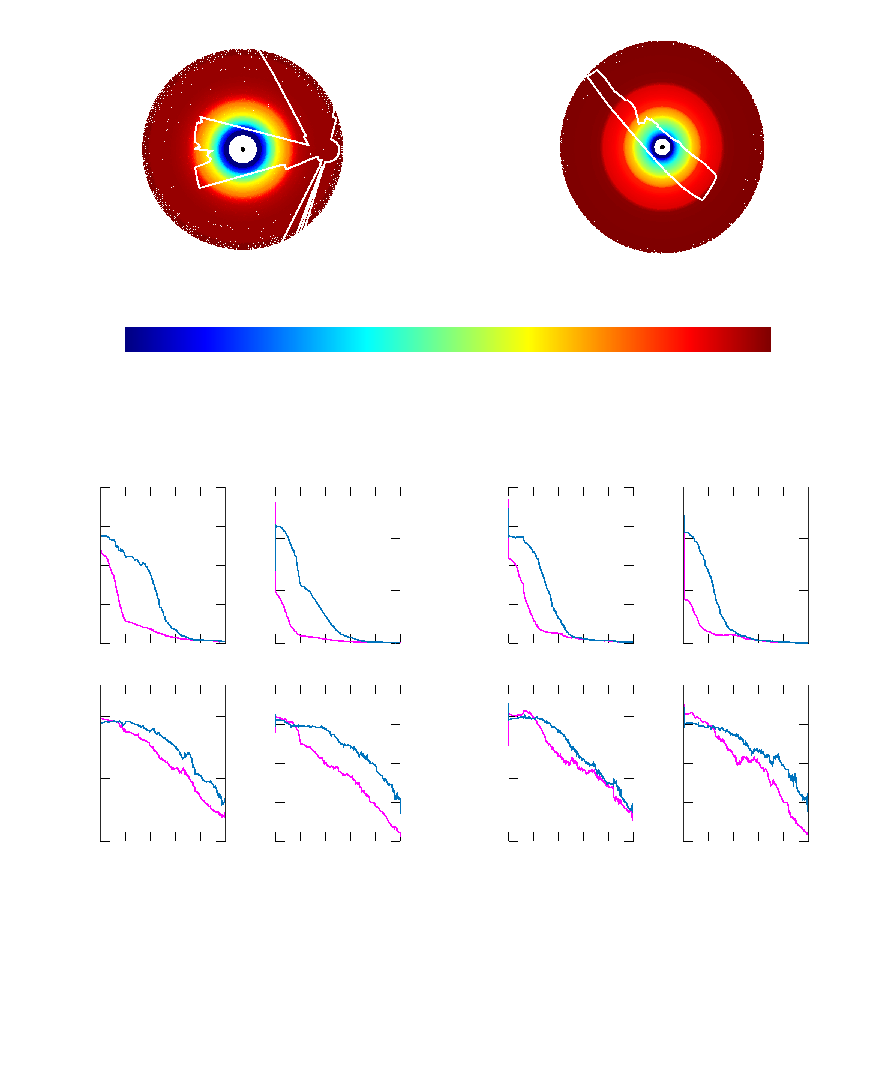
\includegraphics{./figures/parts/02/chapters/05/sections/04/max_range_test}}%
    \gplfronttext
  \end{picture}%
\endgroup

  \vspace{-2cm}
  \caption{\small Πειράματα απόκρισης του σφάλματος εκτίμησης των PLICP
           και FSM σε συνθήκες μειούμενου βεληνεκούς-μέγιστου εύρους
           για τυπική απόκλιση των διαταραχών που επιδρούν στις μετρήσεις του
           φυσικού αισθητήρα όταν $\sigma_R = 0.05$ m. Η διαμόρφωση
           $\Delta_\alpha: (\overline{\delta}_{xy}, \overline{\delta}_{\theta})
           = (0.05,0.174)$ [m,rad]. Η διαμόρφωση $\Delta_\beta:
           (\overline{\delta}_{xy},\overline{\delta}_{\theta}) = (0.20,\pi/4)$
           [m,rad]}
  \label{fig:02_05_04:03}
\end{figure}

Με βάση τα πειραματικά αποτελέσματα παρατηρούμε πως το σφάλμα εκτίμησης
προσανατολισμού του FSM είναι συγκρίσιμο με το ονομαστικό σε συνθήκες
όπου έως το $80\%$ των ακτίνων δεν φέρουν χωρική πληροφορία, σε αντίθεση με το
σφάλμα εκτίμησης θέσης, το οποίο είναι επί της αρχής αντιστρόφως ανάλογο του
ποσοστού των ακτίνων που φέρουν χωρική πληροφορία. Σε χαμηλότερα ποσοστά του
$80\%$ ο FSM επιδεικνύει χαμηλότερα σφάλματα εκτίμησης προσανατολισμού
από τον PLICP, ενώ τα σφάλματα εκτίμησης θέσης του γίνονται μεγαλύτερα από
εκείνα του PLICP όταν περίπου μόνο το $20\%$ των ακτίνων φέρουν ουσιαστική
πληροφορία, παρ' όλο που ο PLICP χρησιμοποιεί αντιστοιχίσεις (και συνεπώς θα
ήταν περισσότερο λογικό να είναι ικανός να αντιστοιχίσει μεμονωμένες περιοχές
των σαρώσεων μεταξύ τους).

Στο σχήμα \ref{fig:02_05_04:04} απεικονίζονται διαφορετικές όψεις της ευρωστίας
της μεθόδου FSM σε πραγματικές συνθήκες. Τα σχήματα της άνω σειράς
αναπαριστούν δύο αρχικές συνθήκες ευθυγράμμισης δισδιάστατων πανοραμικών
σαρώσεων, ενώ της μεσαίας τις τελικές ευθυγραμμίσεις που προέκυψαν μέσω της
εφαρμογής της FSM. Στην αριστερή συνθήκη η τυπική απόκλιση του θορύβου
μέτρησης είναι $\sigma_R = 0.05$ m, ενώ στη δεξιά $\sigma_R = 0.0$ m. Η
τελευταία σειρά εστιάζει σε σημεία ενδιαφέροντος, ήτοι σε περιοχές που εκθέτουν
την ευρωστία της μεθόδου ως προς το θόρυβο μέτρησης, αλλαγές περιβάλλοντος
απρόβλεπτου μέτρου, και ατελείς επικαλύψεις ανάμεσα στις εισόδους.

\begin{figure}[]\centering
  % GNUPLOT: LaTeX picture with Postscript
\begingroup
  \makeatletter
  \providecommand\color[2][]{%
    \GenericError{(gnuplot) \space\space\space\@spaces}{%
      Package color not loaded in conjunction with
      terminal option `colourtext'%
    }{See the gnuplot documentation for explanation.%
    }{Either use 'blacktext' in gnuplot or load the package
      color.sty in LaTeX.}%
    \renewcommand\color[2][]{}%
  }%
  \providecommand\includegraphics[2][]{%
    \GenericError{(gnuplot) \space\space\space\@spaces}{%
      Package graphicx or graphics not loaded%
    }{See the gnuplot documentation for explanation.%
    }{The gnuplot epslatex terminal needs graphicx.sty or graphics.sty.}%
    \renewcommand\includegraphics[2][]{}%
  }%
  \providecommand\rotatebox[2]{#2}%
  \@ifundefined{ifGPcolor}{%
    \newif\ifGPcolor
    \GPcolorfalse
  }{}%
  \@ifundefined{ifGPblacktext}{%
    \newif\ifGPblacktext
    \GPblacktexttrue
  }{}%
  % define a \g@addto@macro without @ in the name:
  \let\gplgaddtomacro\g@addto@macro
  % define empty templates for all commands taking text:
  \gdef\gplbacktext{}%
  \gdef\gplfronttext{}%
  \makeatother
  \ifGPblacktext
    % no textcolor at all
    \def\colorrgb#1{}%
    \def\colorgray#1{}%
  \else
    % gray or color?
    \ifGPcolor
      \def\colorrgb#1{\color[rgb]{#1}}%
      \def\colorgray#1{\color[gray]{#1}}%
      \expandafter\def\csname LTw\endcsname{\color{white}}%
      \expandafter\def\csname LTb\endcsname{\color{black}}%
      \expandafter\def\csname LTa\endcsname{\color{black}}%
      \expandafter\def\csname LT0\endcsname{\color[rgb]{1,0,0}}%
      \expandafter\def\csname LT1\endcsname{\color[rgb]{0,1,0}}%
      \expandafter\def\csname LT2\endcsname{\color[rgb]{0,0,1}}%
      \expandafter\def\csname LT3\endcsname{\color[rgb]{1,0,1}}%
      \expandafter\def\csname LT4\endcsname{\color[rgb]{0,1,1}}%
      \expandafter\def\csname LT5\endcsname{\color[rgb]{1,1,0}}%
      \expandafter\def\csname LT6\endcsname{\color[rgb]{0,0,0}}%
      \expandafter\def\csname LT7\endcsname{\color[rgb]{1,0.3,0}}%
      \expandafter\def\csname LT8\endcsname{\color[rgb]{0.5,0.5,0.5}}%
    \else
      % gray
      \def\colorrgb#1{\color{black}}%
      \def\colorgray#1{\color[gray]{#1}}%
      \expandafter\def\csname LTw\endcsname{\color{white}}%
      \expandafter\def\csname LTb\endcsname{\color{black}}%
      \expandafter\def\csname LTa\endcsname{\color{black}}%
      \expandafter\def\csname LT0\endcsname{\color{black}}%
      \expandafter\def\csname LT1\endcsname{\color{black}}%
      \expandafter\def\csname LT2\endcsname{\color{black}}%
      \expandafter\def\csname LT3\endcsname{\color{black}}%
      \expandafter\def\csname LT4\endcsname{\color{black}}%
      \expandafter\def\csname LT5\endcsname{\color{black}}%
      \expandafter\def\csname LT6\endcsname{\color{black}}%
      \expandafter\def\csname LT7\endcsname{\color{black}}%
      \expandafter\def\csname LT8\endcsname{\color{black}}%
    \fi
  \fi
    \setlength{\unitlength}{0.0500bp}%
    \ifx\gptboxheight\undefined%
      \newlength{\gptboxheight}%
      \newlength{\gptboxwidth}%
      \newsavebox{\gptboxtext}%
    \fi%
    \setlength{\fboxrule}{0.5pt}%
    \setlength{\fboxsep}{1pt}%
\begin{picture}(8000.00,12000.00)%
    \gplgaddtomacro\gplbacktext{%
      \colorrgb{0.15,0.15,0.15}%
      \put(-52,9611){\makebox(0,0)[r]{\strut{}$-32$}}%
      \colorrgb{0.15,0.15,0.15}%
      \put(-52,10173){\makebox(0,0)[r]{\strut{}$-24$}}%
      \colorrgb{0.15,0.15,0.15}%
      \put(-52,10734){\makebox(0,0)[r]{\strut{}$-16$}}%
      \colorrgb{0.15,0.15,0.15}%
      \put(-52,11296){\makebox(0,0)[r]{\strut{}$-8$}}%
      \colorrgb{0.15,0.15,0.15}%
      \put(-52,11857){\makebox(0,0)[r]{\strut{}$0$}}%
      \colorrgb{0.15,0.15,0.15}%
      \put(641,9321){\makebox(0,0){\strut{}$30$}}%
      \colorrgb{0.15,0.15,0.15}%
      \put(1343,9321){\makebox(0,0){\strut{}$50$}}%
      \colorrgb{0.15,0.15,0.15}%
      \put(2045,9321){\makebox(0,0){\strut{}$50$}}%
      \colorrgb{0.15,0.15,0.15}%
      \put(2746,9321){\makebox(0,0){\strut{}$60$}}%
      \colorrgb{0.15,0.15,0.15}%
      \put(3448,9321){\makebox(0,0){\strut{}$70$}}%
    }%
    \gplgaddtomacro\gplfronttext{%
      \colorrgb{0.00,0.00,0.00}%
      \put(1182,12050){\makebox(0,0)[l]{\strut{}Αρχική συνθήκη}}%
      \put(982,9000){\makebox(0,0)[l]{\strut{}$\Delta x = -0.03252$ m}}%
      \put(982,8750){\makebox(0,0)[l]{\strut{}$\Delta y = +0.03603$ m}}%
      \put(982,8500){\makebox(0,0)[l]{\strut{}$\Delta \theta = -0.35689$ rad}}%
    }%
    \gplgaddtomacro\gplbacktext{%
      \colorrgb{0.15,0.15,0.15}%
      \put(4748,9755){\makebox(0,0)[r]{\strut{}$-12$}}%
      \colorrgb{0.15,0.15,0.15}%
      \put(4748,10227){\makebox(0,0)[r]{\strut{}$-10$}}%
      \colorrgb{0.15,0.15,0.15}%
      \put(4748,10699){\makebox(0,0)[r]{\strut{}$-8$}}%
      \colorrgb{0.15,0.15,0.15}%
      \put(4748,11171){\makebox(0,0)[r]{\strut{}$-6$}}%
      \colorrgb{0.15,0.15,0.15}%
      \put(4748,11643){\makebox(0,0)[r]{\strut{}$-4$}}%
      \colorrgb{0.15,0.15,0.15}%
      \put(5116,9299){\makebox(0,0){\strut{}$28$}}%
      \colorrgb{0.15,0.15,0.15}%
      \put(5588,9299){\makebox(0,0){\strut{}$30$}}%
      \colorrgb{0.15,0.15,0.15}%
      \put(6060,9299){\makebox(0,0){\strut{}$32$}}%
      \colorrgb{0.15,0.15,0.15}%
      \put(6531,9299){\makebox(0,0){\strut{}$34$}}%
      \colorrgb{0.15,0.15,0.15}%
      \put(7003,9299){\makebox(0,0){\strut{}$36$}}%
    }%
    \gplgaddtomacro\gplfronttext{%
      \colorrgb{0.00,0.00,0.00}%
      \put(5300,12050){\makebox(0,0)[l]{\strut{}Αρχική συνθήκη}}%
      \put(5200,9000){\makebox(0,0)[l]{\strut{}$\Delta x = -0.02856$ m}}%
      \put(5200,8750){\makebox(0,0)[l]{\strut{}$\Delta y = -0.19805$ m}}%
      \put(5200,8500){\makebox(0,0)[l]{\strut{}$\Delta \theta = -1.31500$ rad}}%
    }%
    \gplgaddtomacro\gplbacktext{%
      \colorrgb{0.15,0.15,0.15}%
      \put(-52,6118){\makebox(0,0)[r]{\strut{}$-32$}}%
      \colorrgb{0.15,0.15,0.15}%
      \put(-52,6399){\makebox(0,0)[r]{\strut{}$-28$}}%
      \colorrgb{0.15,0.15,0.15}%
      \put(-52,6679){\makebox(0,0)[r]{\strut{}$-24$}}%
      \colorrgb{0.15,0.15,0.15}%
      \put(-52,6960){\makebox(0,0)[r]{\strut{}$-20$}}%
      \colorrgb{0.15,0.15,0.15}%
      \put(641,5828){\makebox(0,0){\strut{}$30$}}%
      \colorrgb{0.15,0.15,0.15}%
      \put(1343,5828){\makebox(0,0){\strut{}$50$}}%
      \colorrgb{0.15,0.15,0.15}%
      \put(2045,5828){\makebox(0,0){\strut{}$50$}}%
      \colorrgb{0.15,0.15,0.15}%
      \put(2746,5828){\makebox(0,0){\strut{}$60$}}%
      \colorrgb{0.15,0.15,0.15}%
      \put(3448,5828){\makebox(0,0){\strut{}$70$}}%
    }%
    \gplgaddtomacro\gplfronttext{%
      \colorrgb{0.00,0.00,0.00}%
      \put(982,7200){\makebox(0,0)[l]{\strut{}Τελική ευθυγράμμιση}}%
      \put(982,5500){\makebox(0,0)[l]{\strut{}$\Delta x = -0.00085$ m}}%
      \put(982,5250){\makebox(0,0)[l]{\strut{}$\Delta y = +0.00337$ m}}%
      \put(982,5000){\makebox(0,0)[l]{\strut{}$\Delta \theta = -0.00346$ rad}}%
    }%
    \gplgaddtomacro\gplbacktext{%
      \colorrgb{0.15,0.15,0.15}%
      \put(4748,5596){\makebox(0,0)[r]{\strut{}$-12$}}%
      \colorrgb{0.15,0.15,0.15}%
      \put(4748,6068){\makebox(0,0)[r]{\strut{}$-10$}}%
      \colorrgb{0.15,0.15,0.15}%
      \put(4748,6540){\makebox(0,0)[r]{\strut{}$-8$}}%
      \colorrgb{0.15,0.15,0.15}%
      \put(4748,7011){\makebox(0,0)[r]{\strut{}$-6$}}%
      \colorrgb{0.15,0.15,0.15}%
      \put(4748,7483){\makebox(0,0)[r]{\strut{}$-4$}}%
      \colorrgb{0.15,0.15,0.15}%
      \put(5116,5140){\makebox(0,0){\strut{}$28$}}%
      \colorrgb{0.15,0.15,0.15}%
      \put(5588,5140){\makebox(0,0){\strut{}$30$}}%
      \colorrgb{0.15,0.15,0.15}%
      \put(6060,5140){\makebox(0,0){\strut{}$32$}}%
      \colorrgb{0.15,0.15,0.15}%
      \put(6531,5140){\makebox(0,0){\strut{}$34$}}%
      \colorrgb{0.15,0.15,0.15}%
      \put(7003,5140){\makebox(0,0){\strut{}$36$}}%
    }%
    \gplgaddtomacro\gplfronttext{%
      \colorrgb{0.00,0.00,0.00}%
      \put(5100,7900){\makebox(0,0)[l]{\strut{}Τελική ευθυγράμμιση}}%
      \put(5200,4800){\makebox(0,0)[l]{\strut{}$\Delta x = 0.00643$ m}}%
      \put(5200,4550){\makebox(0,0)[l]{\strut{}$\Delta y = 0.00371$ m}}%
      \put(5200,4300){\makebox(0,0)[l]{\strut{}$\Delta \theta = 0.00194$ rad}}%
    }%
    \gplgaddtomacro\gplbacktext{%
      \colorrgb{0.15,0.15,0.15}%
      \put(42,1815){\makebox(0,0)[r]{\strut{}\scriptsize $-26$}}%
      \colorrgb{0.15,0.15,0.15}%
      \put(42,2479){\makebox(0,0)[r]{\strut{}\scriptsize $-25$}}%
      \colorrgb{0.15,0.15,0.15}%
      \put(42,3143){\makebox(0,0)[r]{\strut{}\scriptsize $-24$}}%
      \colorrgb{0.15,0.15,0.15}%
      \put(412,1263){\makebox(0,0){\strut{}\scriptsize $26$}}%
      \colorrgb{0.15,0.15,0.15}%
      \put(1075,1263){\makebox(0,0){\strut{}\scriptsize $27$}}%
      \colorrgb{0.15,0.15,0.15}%
      \put(1739,1263){\makebox(0,0){\strut{}\scriptsize $28$}}%
    }%
    \gplgaddtomacro\gplfronttext{%
      \colorrgb{0.00,0.00,0.00}%
      \put(909,3496){\makebox(0,0){\strut{}Θόρυβος μέτρησης}}%
    }%
    \gplgaddtomacro\gplbacktext{%
      \colorrgb{0.15,0.15,0.15}%
      \put(2108,2073){\makebox(0,0)[r]{\strut{}\scriptsize $-25$}}%
      \colorrgb{0.15,0.15,0.15}%
      \put(2108,2364){\makebox(0,0)[r]{\strut{}\scriptsize $-24$}}%
      \colorrgb{0.15,0.15,0.15}%
      \put(2108,2656){\makebox(0,0)[r]{\strut{}\scriptsize $-23$}}%
      \colorrgb{0.15,0.15,0.15}%
      \put(2518,1635){\makebox(0,0){\strut{}\scriptsize $31$}}%
      \colorrgb{0.15,0.15,0.15}%
      \put(3100,1635){\makebox(0,0){\strut{}\scriptsize $33$}}%
      \colorrgb{0.15,0.15,0.15}%
      \put(3683,1635){\makebox(0,0){\strut{}\scriptsize $35$}}%
    }%
    \gplgaddtomacro\gplfronttext{%
    }%
    \gplgaddtomacro\gplbacktext{%
      \colorrgb{0.15,0.15,0.15}%
      \put(4168,1901){\makebox(0,0)[r]{\strut{}\scriptsize $-6$}}%
      \colorrgb{0.15,0.15,0.15}%
      \put(4168,2464){\makebox(0,0)[r]{\strut{}\scriptsize $-5$}}%
      \colorrgb{0.15,0.15,0.15}%
      \put(4168,3027){\makebox(0,0)[r]{\strut{}\scriptsize $-4$}}%
      \colorrgb{0.15,0.15,0.15}%
      \put(4706,1231){\makebox(0,0){\strut{}\scriptsize $32$}}%
      \colorrgb{0.15,0.15,0.15}%
      \put(5269,1231){\makebox(0,0){\strut{}\scriptsize $33$}}%
      \colorrgb{0.15,0.15,0.15}%
      \put(5831,1231){\makebox(0,0){\strut{}\scriptsize $34$}}%
    }%
    \gplgaddtomacro\gplfronttext{%
      \colorrgb{0.00,0.00,0.00}%
      \put(2457,3589){\makebox(0,0)[l]{\strut{}Στοιχεία υψηλής συχνότητος}}%
    }%
    \gplgaddtomacro\gplbacktext{%
      \colorrgb{0.15,0.15,0.15}%
      \put(6228,1704){\makebox(0,0)[r]{\strut{}\scriptsize $-8$}}%
      \colorrgb{0.15,0.15,0.15}%
      \put(6228,2165){\makebox(0,0)[r]{\strut{}\scriptsize $-7$}}%
      \colorrgb{0.15,0.15,0.15}%
      \put(6228,2626){\makebox(0,0)[r]{\strut{}\scriptsize $-6$}}%
      \colorrgb{0.15,0.15,0.15}%
      \put(6228,3087){\makebox(0,0)[r]{\strut{}\scriptsize $-5$}}%
      \colorrgb{0.15,0.15,0.15}%
      \put(6260,1406){\makebox(0,0){\strut{}\scriptsize $30$}}%
      \colorrgb{0.15,0.15,0.15}%
      \put(6721,1406){\makebox(0,0){\strut{}\scriptsize $31$}}%
      \colorrgb{0.15,0.15,0.15}%
      \put(7182,1406){\makebox(0,0){\strut{}\scriptsize $32$}}%
      \colorrgb{0.15,0.15,0.15}%
      \put(7643,1406){\makebox(0,0){\strut{}\scriptsize $33$}}%
    }%
    \gplgaddtomacro\gplfronttext{%
      \colorrgb{0.00,0.00,0.00}%
      \put(7089,3353){\makebox(0,0){\strut{}Απούσες αντιστοιχίες}}%
    }%
    \gplbacktext
    \put(0,0){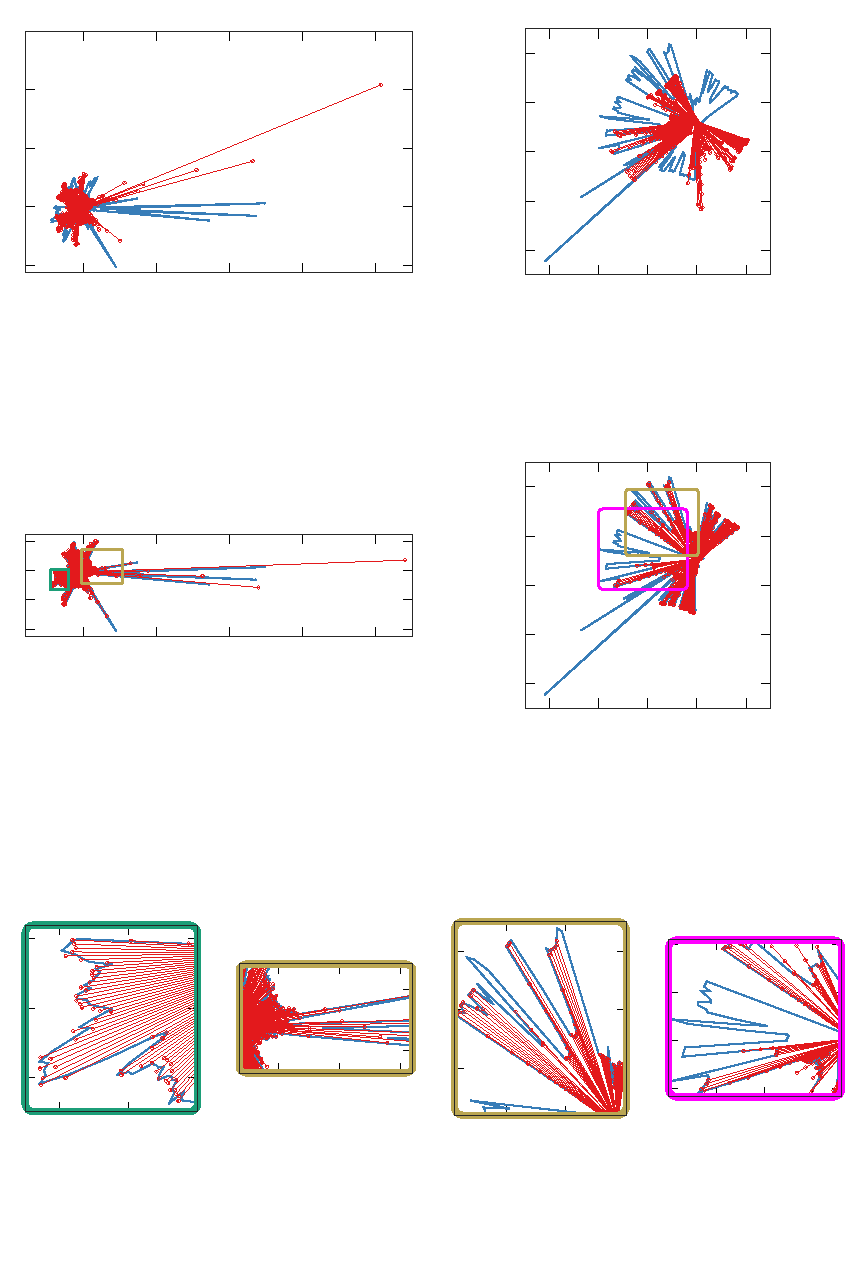
\includegraphics{./figures/parts/02/chapters/05/sections/04/from_video}}%
    \gplfronttext
  \end{picture}%
\endgroup

  \vspace{-1cm}
  \caption{\small Παραδείγματα ευθυγράμμισης σαρώσεων που εκθέτουν τις αρετές
           του FSM σε καταστάσεις πραγματικών συνθηκών: ο FSM
           είναι ταυτόχρονα εύρωστος σε θόρυβο μέτρησης, απρόβλεπτα μεγάλες
           αλλαγές στο περιβάλλον από το οποίο συλλαμβάνονται οι σαρώσεις
           εισόδου του, και σε συνθήκες μερικής επικάλυψης}
  \label{fig:02_05_04:04}
\end{figure}
